\begin{figure}[htbp]
\centering
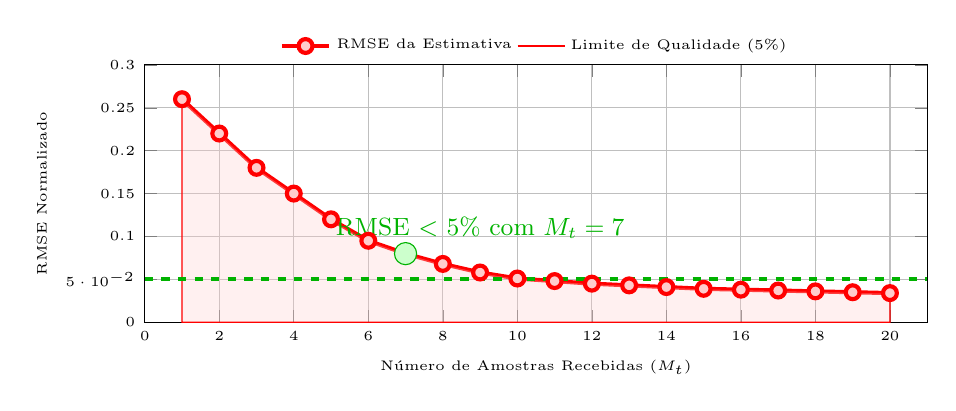
\begin{tikzpicture}
\begin{axis}[
    width=0.95\textwidth,
    height=0.40\textwidth,
    xlabel={Número de Amostras Recebidas ($M_t$)},
    ylabel={RMSE Normalizado},
    grid=major,
    legend style={at={(0.5,-0.15)}, anchor=north, legend columns=2},
    xmin=0, xmax=21,
    ymin=0, ymax=0.3,
    xtick={0,2,4,6,8,10,12,14,16,18,20},
    ytick={0,0.05,0.10,0.15,0.20,0.25,0.30},
    tick label style={font=\tiny},
    label style={font=\tiny},
    legend style={font=\tiny},
    legend cell align=left,
    legend style={
        at={(0.5,1.)},
        anchor=south,
        legend columns=3,
        font=\tiny,
        draw=none
    },
    % title={Convergência do RMSE Normalizado da Estimativa Nutricional},
    % title style={font=\large\bfseries, yshift=8pt}
]

% RMSE vs Amostras Recebidas
\addplot[red, line width=1.5pt, mark=*, mark size=2.5pt, mark options={fill=red!20}] coordinates {
    (1, 0.26) (2, 0.22) (3, 0.18) (4, 0.15) (5, 0.12)
    (6, 0.095) (7, 0.080) (8, 0.068) (9, 0.058) (10, 0.051)
    (11, 0.048) (12, 0.045) (13, 0.043) (14, 0.041) (15, 0.039)
    (16, 0.038) (17, 0.037) (18, 0.036) (19, 0.035) (20, 0.034)
};
\addlegendentry{RMSE da Estimativa}

% Área sob a curva
\addplot[red, fill=red!20, fill opacity=0.3] coordinates {
    (1, 0) (1, 0.26) (2, 0.22) (3, 0.18) (4, 0.15) (5, 0.12)
    (6, 0.095) (7, 0.080) (8, 0.068) (9, 0.058) (10, 0.051)
    (11, 0.048) (12, 0.045) (13, 0.043) (14, 0.041) (15, 0.039)
    (16, 0.038) (17, 0.037) (18, 0.036) (19, 0.035) (20, 0.034) (20, 0)
} \closedcycle;

% Linha de limite 5%
\addplot[green!70!black, dashed, line width=1.5pt] coordinates {
    (0, 0.05) (21, 0.05)
};
\addlegendentry{Limite de Qualidade (5\%)}

% Ponto onde atinge <5%
\addplot[only marks, mark=*, mark size=4pt, color=green!70!black, fill=green!20] coordinates {
    (7, 0.080)
};

% Anotação
\node[draw, fill=green!10, rounded corners, font=\tiny, align=left, anchor=north east] at (0.98, 0.98) {
    Limite de 5\% atingido\\
    com $M_t = 7$ amostras\\
    Convergência rápida do erro
};

% Anotação do ponto
\node[font=\small, color=green!70!black] at (axis cs:9,0.11) {RMSE $<$ 5\% com $M_t=7$};

\end{axis}
\end{tikzpicture}
\caption{Convergência do RMSE normalizado da estimativa nutricional em função do número de amostras recebidas. Observa-se que o erro atinge o limite de qualidade de 5\% com apenas 7 amostras.}
\label{fig:convergencia_rmse}
\end{figure}
